\documentclass[conference]{IEEEtran}

\usepackage{cmap}
\usepackage[utf8]{inputenc}
\usepackage[english]{babel}

\usepackage{indentfirst} 
\usepackage{amsmath,amssymb,amscd,amsthm}
\usepackage{mathtools}
%\usepackage{empheq}
%\newcommand*{\widebox}[2][0.5em]{\fbox{\hspace{#1}$\displaystyle #2$\hspace{#1}}}
%\usepackage{longtable}
\usepackage{multirow}
\usepackage{multicol}

\usepackage{graphicx}
\usepackage{caption}
\usepackage{subcaption}
\usepackage{siunitx}

\usepackage{enumitem}

\renewcommand{\sfdefault}{cmss}
\renewcommand{\rmdefault}{cmr}
\renewcommand{\ttdefault}{cmt}

\usepackage{tikz}
\usetikzlibrary{shapes,shapes.geometric,arrows,fit,calc,positioning,automata}
\usetikzlibrary{arrows}
\usetikzlibrary{shapes.multipart}
\usetikzlibrary{decorations.pathreplacing}
\usetikzlibrary{patterns}
\usetikzlibrary{arrows.meta}

\usepackage[e]{esvect}		
													
\usepackage{xcolor}
\definecolor{darkblue}{rgb}{0,0,.6}
\definecolor{Purplemountainmajesty}{RGB}{150, 120, 182}
\definecolor{prpl}{RGB}{150, 120, 182}

\interdisplaylinepenalty=2500

\pdfcompresslevel=9
\pdfobjcompresslevel=9

\usepackage{cite}
%\usepackage[breaklinks,pdftex,hyperindex,unicode]{hyperref}	
%\hypersetup{
%  pdftitle           = {IEEE 802.11ax},
%  pdfauthor          = {Didenko Andre},
%  pdfsubject         = {IEEE 802.11ax},
%  pdfstartview       = {FitH},
%  pdfborder          = {0 0 0},
%  bookmarksopen      = true,
%  bookmarksnumbered  = true,
%  bookmarksopenlevel = 2,
%  colorlinks = true,     
%  		linkcolor  = black, 
%  		urlcolor = black,
%        citecolor = black
%}

%!!!conflicting order of packages
%\usepackage{extarrows}
% fix \ordinarycolon
\edef\ordinarycolon{\mathchar\the\mathcode`:}

%\usepackage{todonotes}
%\presetkeys{todonotes}{inline, color=Purplemountainmajesty}{}

%%% my macros

%% Math fonts
\newcommand{\bbA}{\mathbb{A}}
\newcommand{\bbB}{\mathbb{B}}
\newcommand{\bbC}{\mathbb{C}} % комплексные числа
\newcommand{\bbD}{\mathbb{D}}
\newcommand{\bbE}{\mathbb{E}} 
\newcommand{\bbF}{\mathbb{F}}
\newcommand{\bbG}{\mathbb{G}}
\newcommand{\bbH}{\mathbb{H}}
\newcommand{\bbI}{\mathbb{I}}
\newcommand{\bbJ}{\mathbb{J}}
\newcommand{\bbK}{\mathbb{K}}
\newcommand{\bbL}{\mathbb{L}}
\newcommand{\bbM}{\mathbb{M}}
\newcommand{\bbN}{\mathbb{N}} %натуральные числа
\newcommand{\bbO}{\mathbb{O}}
\newcommand{\bbP}{\mathbb{P}}
\newcommand{\bbQ}{\mathbb{Q}} % рациональные числа
\newcommand{\bbR}{\mathbb{R}} % действительные числа
\newcommand{\bbS}{\mathbb{S}}
\newcommand{\bbT}{\mathbb{T}}
\newcommand{\bbU}{\mathbb{U}}
\newcommand{\bbV}{\mathbb{V}}
\newcommand{\bbW}{\mathbb{W}}
\newcommand{\bbX}{\mathbb{X}}
\newcommand{\bbY}{\mathbb{Y}}
\newcommand{\bbZ}{\mathbb{Z}} %целые числа

%Матожидание и Дисперсия. 
\newcommand{\ccM}{\mathcal{M}}
\newcommand{\ccD}{\mathcal{D}}

% Привычное написание букв каппа, эпсилон и фи и знаков "больше, или равно", "меньше, или равно", пустого множества
\renewcommand{\kappa}{\varkappa }
\renewcommand{\epsilon}{\varepsilon}
\renewcommand{\phi}{\varphi}
\renewcommand{\leq}{\leqslant}
\renewcommand{\geq}{\geqslant}
\renewcommand{\emptyset}{\varnothing}

%Возможно правильная расстановка пробелов в кванторах - НЕ ИСПОЛЬЗУЙТЕ НИ ЗА ЧТО НА СВЕТЕ, ЛУЧШЕ РУКАМИ.
\newcommand{\fa}{\quad\forall}%renewcommand возможно из-за package fontawesome, который добавляет кучу красивых символов (смайлики, рожицы, значки)
\newcommand{\ex}{\quad\exists}

%Множества с чертой:
\newcommand{\bboR}{\overline{\mathbb{R}}}
\newcommand{\bboC}{\overline{\mathbb{C}}}

%Проколотая окрестность
\newcommand{\dneio}[2]{\overset{\raisebox{0pt}[0pt][0pt]{$\scriptscriptstyle\circ$}}{O}_{#1}({#2})}
\newcommand{\dnei}[1]{\overset{\raisebox{0pt}[0pt][0pt]{$\scriptscriptstyle\circ$}}{O}({#1})}
\newcommand{\coci}[2][]{\overset{\raisebox{0pt}[0pt][0pt]{$\scriptscriptstyle\circ$}}{C^{#1}}{#2}}

% Полная производная
\newcommand{\D}[2]{\frac{d{#1}}{d{#2}}}

% Частная производная
\newcommand{\pd}[2]{\frac{\partial{#1}}{\partial{#2}}}

%%%%%%%%%%%%%%%%%%%%%%%%%%%%%%%%%%%%%%%%%%

% Действительная и мнимая части
\def\Re{\mathop{\mathrm{Re}}\nolimits}
\def\Im{\mathop{\mathrm{Im}}\nolimits}

%Ядро отображения
\def\Ker{\mathop{\mathrm{Ker}}\nolimits}

%Внутренность множества.
\DeclareMathOperator*{\interior}{int} % * предполагает использование \limits

% Носитель
\def\supp{\mathop{\mathrm{supp}}\limits}

% Дивергенция
\def\Div{\mathop{\mathrm{div}}\nolimits}

% Ротор
\def\rot{\mathop{\mathrm{rot}}\nolimits}

% Градиент
\def\grad{\mathop{\mathrm{grad}}\limits}

% Градиент
\def\argmax{\mathop{\mathrm{argmax}}\limits}

% Константа
\def\const{\mathop{\mathrm{const}}\nolimits}

% Ранг
\def\rg{\mathop{\mathrm{rg}}\nolimits}

%% Вычет
\def\res{\mathop{\rm res}\limits}

%% Расстояние
\def\dist{\mathop{\rm dist}\limits}

%% Ковариация
\def\cov{\mathop{\rm cov}\limits}

%% Интеграл в смысле главного значения
\def\v.p.{\mathop{\rm v.p.}\nolimits}

%Гиперболические функции
\def\sh{\mathop{\rm sh}\nolimits}
\def\ch{\mathop{\rm ch}\nolimits}
\def\th{\mathop{\rm th}\nolimits}

%Арктангенс
\def\arctg{\mathop{\rm arctg}\nolimits}

%Обратные гиперболические функции 
\def\arsh{\mathop{\rm arsh}\nolimits}
\def\arch{\mathop{\rm arch}\nolimits}
\def\arth{\mathop{\rm arth}\nolimits}

%%%%%%%%%%%%%%%%%%%%%%%%%%%%%%%%%%%%%%%%%%

% Крупная хи
\newcommand{\bigchi}{\text{\scalebox{1.5}{$\chi$}}}

% Римские цифры
\makeatletter
\newcommand*{\rom}[1]{\expandafter\@slowromancap\romannumeral #1@}
\makeatother

%% Text fomats
\newcommand{\tbi}[1]{\textbf{\textit{#1}}}

%% Сокращение для одной штуки

\newcommand{\Gp}{(\partial G)^{+}}

\newcommand{\Gm}{(\partial G)^{-}}










%%Это перешло сюда по наследству от теорфиза, пусть будет, мало ли. 

% Скобки (высокие)
\newcommand{\brc}[1]{\left ( {#1} \right )}

% Скобки фигурные (высокие)
\newcommand{\brcr}[1]{\left\{ {#1} \right\}}

% Скобки квадратные (высокие)
\newcommand{\brs}[1]{\left [ {#1} \right ]}

% Усреднение
\newcommand{\avg}[1]{\langle{#1}\rangle}

% Усреднение (высокое)
\newcommand{\avgh}[1]{\left\langle{#1}\right\rangle}

% Бра-вектор
\newcommand{\bra}[1]{\left\langle{#1}\right|}

% Кет-вектор
\newcommand{\ket}[1]{\left|{#1}\right\rangle}

% Скалярное произведение
\newcommand{\bk}[2]{\langle{#1}|{#2}\rangle}

% Скалярное произведение (высокое)
\newcommand{\bkh}[2]{\left\langle{#1}|{#2}\right\rangle}

% Проектор
\newcommand{\proj}[2]{\ket{#1}\bra{#2}}

% Матричный элемент
\newcommand{\bfk}[3]{\langle{#1}|{#2}|{#3}\rangle}

% Матричный элемент (высокий)
\newcommand{\bfkh}[3]{\left\langle{#1}\left|{#2}\right|{#3}\right\rangle}

% Модуль
\providecommand{\abs}[1]{\left\lvert{#1}\right\rvert}

% Норма
\providecommand{\norm}[1]{\lVert#1\rVert}

% След матрицы

\def\sp{\mathop{\mathrm{sp}}\nolimits}


\begin{document}
\IEEEoverridecommandlockouts

\title{%IEEE~802.11ax Uplink Scheduler to Minimize Delay: a Classic Problem with New Constraints
Scheduling Problem for OFDMA Uplink \\in IEEE 802.11ax Networks
\thanks{The research was supported by the Russian Science Foundation (agreement No 16-19-10687).}}

\author{
\IEEEauthorblockN{Dmitry Bankov, Andre Didenko, Evgeny Khorov, Vyacheslav Loginov, Andrey Lyakhov}
\IEEEauthorblockA{Institute for Information Transmission Problems, Russian Academy of Sciences, Moscow, Russia\\
Email: \{bankov, dida, khorov, loginov, lyakhov\}@iitp.ru}
}

\maketitle

\begin{abstract}
In the modern world to have a high-speed Internet connection is already more a necessity than a luxury. 
But in \textcolor{prpl}{current reality}, a wireless connection does not work well in dense networks. 
So new generation of Wi-Fi devices is coming due to development of the standard IEEE 802.11ax, which should be publicly released in a couple of years. 
This new standard has the challenging goal of improving performance indicators such as throughput per user, spectral efficiency, etc. 
It takes the best of Wi-Fi and adds technology from cellular technologies, hence combination of both technologies will be key in designing the best performing IEEE 802.11ax solutions. 
The most ground-breaking technology taken from cellular networks is OFDMA which gives opportunity for an Access Point to serve several users simultaneously with frequency division. 
It gives rise to the problem of resource planning in Wi-Fi networks with new constraints.
In this paper we investigate the scheduling problem, study peculiarities of this technology union in Wi-Fi and develop a new type of schedulers.
Also we show a way to adapt traditional schedulers to  IEEE 802.11ax networks.
\end{abstract}

\begin{IEEEkeywords}
Wi-Fi, IEEE 802.11ax, High Efficiency WLAN, OFDMA, Scheduling
\end{IEEEkeywords}

\section{Introduction}

Wireless networks have become indispensable in the modern world.
Nowadays, Wireless Local Area Network (WLAN) is believed to be the most popular technology for information transmission. 
It is not surprising. 
People can go online literally anywhere: in a restaurant, cafe, shopping center, park, public transport, airport, at work and, of course, at home. 
\textcolor{prpl}{The main concern is just to be within the range of the approachable Wi-Fi Access Point (AP).} 
Such popularity of this technology has led to the problem of congestion of Wi-Fi networks, when one network interrupts the signal of another. 
To cope with this and many other circumstances, IEEE 802 LAN/MAN Standard committee is developing a new amendment for Wi-Fi standard: IEEE 802.11ax (further in the paper referred to as 11ax). 

This amendment provides various ways to improve the efficiency of Wi-Fi, some of which are borrowed from cellular technology.
One of such most significant enhancements of 11ax is the usa\-ge of Orthogonal Frequency-Division Multiple Access (OFDMA). 
It allows a Wi-Fi AP to service several stations (STAs) simultaneously, to better cope with fading and, in case of uplink transmission, to improve the spectral power density. 
In a cost of that the 11ax will provide only a flexible framework so developers need to determine effective schedule algorithms for this OFDMA system while its effectiveness fully depends on the resource management.   

The resource management problem itself has been studied well in other OFDMA-systems, like cellular networks, for which this technology is not new. 
We can borrow some ideas from them as well as 11ax borrows OFDMA technology from cellular networks. 
We can implement 11ax Wi-Fi adaptation for schedulers known from mobile networks considering OFDMA features in Wi-Fi which impose some difficult constraints.  

In this paper, we study problems that arise while developing the schedulers for Uplink (UL) in 11ax networks. The main goal of this paper is to introduce our method to allocate resources in 11ax networks. We also show how to implement this method for some well-investigated schedulers. 
Moreover, \textcolor{prpl}{we present a new type of schedulers, which we also offer to a reader's attention}.

The rest of the paper is organized as follows.
Section~\ref{sec:features} briefly describes the basic OFDMA features in 11ax networks.
Section~\ref{sec:related} provides an overview on related papers.
Network scenario is shown in Section~\ref{sec:scenario} and problem statement is also given there.
In Section~\ref{sec:scheduling}, we cover scheduling problem in 11ax networks and describe main principles of developed 11ax schedulers.
In Section~\ref{sec:adaptations}, we illustrate a way to adapt well-known schedulers for 11ax networks.
In Section~\ref{sec:numerical}, we demonstrate and discuss numerical results. 
Section~\ref{sec:conclusion} concludes the paper.
\section{OFDMA features in 11ax}
\label{sec:features}

Data transmission in Wi-Fi with OFDMA has a number of non-trivial peculiarities which make it different from data transmission in 4G technology, although it also uses OFDMA.

\subsection{Channelization in 802.11ax}
The available channel can be split into sets of OFDMA subcarriers called resource units (RUs).
The 11ax defines RUs that consist of 26, 52, 106, 242, 484, 996 and $2\times996$ OFDM tones.
The set of available RUs depends on the channel width, e.g., in a \SI{40}{\MHz} channel the STAs can use RUs with up to 484 tones.
A wide RUs can be split into narrower RUs: 52-tone, 106-tone RU and 484-tone RUs can be split in two approximately twice-narrower RUs from available set, while 242-tone and 996-tone RUs are split into three RBs (see Fig.~\ref{fig:resource_units}).
Note that these the divisions of the RUs can be made independently from others. 

The scheduler can allocate only one RU to a STA, but it can vary the RU size for each STA according to the aforementioned limitations.
In other words we have 37 26-tone RUs and certain groups of 2, 4, 9, 18 or all 37 of them can be united in order to obtain larger RUs.
According to the standard, such a limitation appears because of the need to have service tones next to each allocated RU of any size. 
Note that position of these divided RBs is declared in standard and cannot be arbitrary.
For example, as shown at Fig.~\ref{fig:resource_units} two first RUs are united in one 52-tone RU, but we cannot unite the second and the third ones.


\begin{figure}[tb]
	\centering
	\begin{scaletikzpicturetowidth}{0.5\textwidth}
	\begin{tikzpicture}[scale = \tikzscale]
	
	%\tikzset{primarynode/.style={isosceles triangle, draw, inner sep=0pt, anchor=left corner, shape border rotate=90, font=\small, fill=gray!25, isosceles triangle stretches, minimum height = 0.8cm,minimum width=0.36cm}}
	
	%\node [primarynode] at (-0.36,4.0) {1};
		
	\draw [line width=0.2mm] (0.00, 0.00) rectangle (9.00, 0.80);
	\node [text width=1.5cm, align=center] at (4.0,  0.4) {484};
	\node [text width=1.5cm, align=center] at (5.0,  0.4) {tones};
	
	\draw [line width=0.2mm] (0.00, 1.0) rectangle (4.50, 1.8);
	\draw [line width=0.2mm] (4.50, 1.0) rectangle (9.00, 1.8);
	\node [text width=1.5cm, align=center] at (2.5,  1.4) {242};
	\node [text width=1.5cm, align=center] at (7.0,  1.4) {242};
	
	\draw [line width=0.2mm] (0.00, 2.0) rectangle (2.00, 2.8);
	\draw [line width=0.2mm] (2.00, 2.0) rectangle (2.50, 2.8);
	\draw [line width=0.2mm] (2.50, 2.0) rectangle (4.50, 2.8);
	\draw [line width=0.2mm] (4.50, 2.0) rectangle (6.50, 2.8);
	\draw [line width=0.2mm] (6.50, 2.0) rectangle (7.00, 2.8);
	\draw [line width=0.2mm] (7.00, 2.0) rectangle (9.00, 2.8);
	\node [text width=1.5cm, align=center] at (1.0,  2.4) {106};
	\node [text width=1.5cm, align=center] at (2.25, 2.4) {26};
	\node [text width=1.5cm, align=center] at (3.5,  2.4) {106};
	\node [text width=1.5cm, align=center] at (5.5,  2.4) {106};
	\node [text width=1.5cm, align=center] at (6.75, 2.4) {26};
	\node [text width=1.5cm, align=center] at (8.0,  2.4) {106};
	
	\draw [line width=0.2mm] (0.00, 3.0) rectangle (1.00, 3.8);
	\draw [line width=0.2mm] (1.00, 3.0) rectangle (2.00, 3.8);
	\draw [line width=0.2mm] (2.00, 3.0) rectangle (2.50, 3.8);
	\draw [line width=0.2mm] (2.50, 3.0) rectangle (3.50, 3.8);
	\draw [line width=0.2mm] (3.50, 3.0) rectangle (4.50, 3.8);
	\draw [line width=0.2mm] (4.50, 3.0) rectangle (5.50, 3.8);
	\draw [line width=0.2mm] (5.50, 3.0) rectangle (6.50, 3.8);
	\draw [line width=0.2mm] (6.50, 3.0) rectangle (7.00, 3.8);
	\draw [line width=0.2mm] (7.00, 3.0) rectangle (8.00, 3.8);
	\draw [line width=0.2mm] (8.00, 3.0) rectangle (9.00, 3.8);
	\node [text width=1.5cm, align=center] at (0.5,  3.4) {52};
	\node [text width=1.5cm, align=center] at (1.5,  3.4) {52};
	\node [text width=1.5cm, align=center] at (2.25, 3.4) {26};
	\node [text width=1.5cm, align=center] at (3.0,  3.4) {52};
	\node [text width=1.5cm, align=center] at (4.0,  3.4) {52};
	\node [text width=1.5cm, align=center] at (5.0,  3.4) {52};
	\node [text width=1.5cm, align=center] at (6.0,  3.4) {52};
	\node [text width=1.5cm, align=center] at (6.75, 3.4) {26};
	\node [text width=1.5cm, align=center] at (7.5,  3.4) {52};
	\node [text width=1.5cm, align=center] at (8.5,  3.4) {52};
	
	\draw [line width=0.2mm] (0.00, 4.0) rectangle (0.50, 4.8);
	\draw [line width=0.2mm] (0.50, 4.0) rectangle (1.00, 4.8);
	\draw [line width=0.2mm] (1.00, 4.0) rectangle (1.50, 4.8);
	\draw [line width=0.2mm] (1.50, 4.0) rectangle (2.00, 4.8);
	\draw [line width=0.2mm] (2.00, 4.0) rectangle (2.50, 4.8);
	\draw [line width=0.2mm] (2.50, 4.0) rectangle (3.00, 4.8);
	\draw [line width=0.2mm] (3.00, 4.0) rectangle (3.50, 4.8);
	\draw [line width=0.2mm] (3.50, 4.0) rectangle (4.00, 4.8);
	\draw [line width=0.2mm] (4.00, 4.0) rectangle (4.50, 4.8);
	\draw [line width=0.2mm] (4.50, 4.0) rectangle (5.00, 4.8);
	\draw [line width=0.2mm] (5.00, 4.0) rectangle (5.50, 4.8);
	\draw [line width=0.2mm] (5.50, 4.0) rectangle (6.00, 4.8);
	\draw [line width=0.2mm] (6.00, 4.0) rectangle (6.50, 4.8);
	\draw [line width=0.2mm] (6.50, 4.0) rectangle (7.00, 4.8);
	\draw [line width=0.2mm] (7.00, 4.0) rectangle (7.50, 4.8);
	\draw [line width=0.2mm] (7.50, 4.0) rectangle (8.00, 4.8);
	\draw [line width=0.2mm] (8.00, 4.0) rectangle (8.50, 4.8);
	\draw [line width=0.2mm] (8.50, 4.0) rectangle (9.00, 4.8);
	\node [text width=1.5cm, align=center] at (0.25, 4.4) {26};
	\node [text width=1.5cm, align=center] at (0.75, 4.4) {26};
	\node [text width=1.5cm, align=center] at (1.25, 4.4) {26};
	\node [text width=1.5cm, align=center] at (1.75, 4.4) {26};
	\node [text width=1.5cm, align=center] at (2.25, 4.4) {26};
	\node [text width=1.5cm, align=center] at (2.75, 4.4) {26};
	\node [text width=1.5cm, align=center] at (3.25, 4.4) {26};
	\node [text width=1.5cm, align=center] at (3.75, 4.4) {26};
	\node [text width=1.5cm, align=center] at (4.25, 4.4) {26};
	\node [text width=1.5cm, align=center] at (4.75, 4.4) {26};
	\node [text width=1.5cm, align=center] at (5.25, 4.4) {26};
	\node [text width=1.5cm, align=center] at (5.75, 4.4) {26};
	\node [text width=1.5cm, align=center] at (6.25, 4.4) {26};
	\node [text width=1.5cm, align=center] at (6.75, 4.4) {26};
	\node [text width=1.5cm, align=center] at (7.25, 4.4) {26};
	\node [text width=1.5cm, align=center] at (7.75, 4.4) {26};
	\node [text width=1.5cm, align=center] at (8.25, 4.4) {26};
	\node [text width=1.5cm, align=center] at (8.75, 4.4) {26};
	
	%\node [text width=1.5cm, align=center] at (4.5, 8.8) {DC};
	%\draw [line width=0.5mm, dashed] (4.5, 1.0) -- (4.5, 8.5);
	
	%\draw [line width=0.5mm, dashed] (0.0, 4.0) -- (0.0, 8.5);
	%\draw [line width=0.5mm, dashed] (2.0, 4.0) -- (2.0, 8.5);
	%\draw [line width=0.5mm, dashed] (2.5, 4.0) -- (2.5, 8.5);
	%\draw [line width=0.5mm, dashed] (4.5, 4.0) -- (4.5, 8.5);
	
	\end{tikzpicture}
	\end{scaletikzpicturetowidth}
	\caption{\label{fig:resource_units} RU locations in \SI{40}{\MHz} channel}
	\vspace{-0.5em}
\end{figure}

The size of an RU determines the set of modulation-coding schemes (MCSs) that can be used for transmission in the RU.
For example, the standard prohibits usage of the novel 1024-QAM in small RUs.
At the same time, for each RU width, the standard defines the minimal receiver sensitivity to signal transmitted with a specific MCS, and the faster the MCS, the higher is the sensitivity threshold.
As the result, a STA cannot use high-speed MCSs if it has poor channel conditions.	

A wider RU does not necessarily mean that the STA transmits at greater speed.
A STA uses the same transmission power both for wide and narrow RUs, which results in greater signal-to-noise ratio ($SNR$) values for narrow RUs.
As the result, in a narrow RU it can use higher MCSs which can yield greater total transmission rate. 
Data rates of MCSs used in the 11ax are indicated in Table~\ref{table:RUdatarate}. 

\begin{table}[t]
	{\centering
		\caption{\label{table:RUdatarate} Data rate in different RU at each MCS in Mbps}
		\resizebox{\columnwidth}{!}{
			\setlength\tabcolsep{1.5pt} % default value: 6pt
			\begin{tabular}{|c|c|c|c|c|c|c|c|}
				\hline
				&\scriptsize\textbf{MCS}	& \scriptsize26-tone  & \scriptsize52-tone  & \scriptsize106-tone  & \scriptsize242-tone  & \scriptsize484-tone  & \scriptsize996-tone  \\
				\hline
				1 & BPSK, 1/2		&0.8	&1.7	&3.5	&8.1 & 16.3 &34		\\
				2 & QPSK, 1/2		&1.7	&3.3	&7.1	&16.3 & 32.5 &68.1	\\
				3 & QPSK, 3/4		&2.5	&5	&10.6	&24.4 & 48.8 &102.1		\\
				4 & 16-QAM, 1/2		&3.3	&6.7	&14.2	&32.5 & 65 &136.1	\\
				5 & 16-QAM, 3/4		&5	&10	&21.3	&48.8 & 97.5 &204.2			\\
				6 & 64-QAM, 2/3		&6.7	&13.3	&28.3	&65 & 130 &272.2	\\
				7 & 64-QAM, 3/4		&7.5	&15	&31.9	&73.1 & 146.3 &306.3	\\
				8 & 64-QAM, 5/6		&8.3	&16.7	&35.4	&81.3 & 162.5 &340.3	\\
				9 & 256-QAM, 3/4	&10	&20	&42.5	&97.5 & 195 &408.3		     	\\
				10 & 256-QAM, 5/6	&11.1	&22.2	&47.2	&108.3 & 216.7 &453.7	\\
				11 & 1024-QAM, 3/4	& --	&--	&--	&121.9 & 243.8 &510.4		 	\\
				12 & 1024-QAM, 5/6 	& --	&--	&--	&135.4 & 270.8 &576.1		 	\\
				\hline
			\end{tabular}
		}
	}
\end{table}	

Another problem is that in order to enable the AP to successfully receive the signal from several STAs, these STAs should transmit with such power that the incoming signal is the same at the AP.
This makes OFDMA usage be possible. 
This implies all STAs to transmit with the same synchronized MCS. 
There is one exception in this rule: when we use 1024-QAM in a RU bigger than 20 MHz we still can transmit data in smaller ones with 256-QAM. 

Such constraints complicate scheduling problem in 11ax networks.

\subsection{Data Transmission Sequence}

All transmissions inside one OFDMA frame must start and finish at the same time. 
There is no problem in downlink (DL) to manage this because an OFDMA frame here is generated by the AP. 
But to synchronize UP and to organize data transmission process in UL with OFDMA, the AP transmits novel Trigger Frames (TF). in which it includes the scheduling information (see Fig. \ref{fig:transmission}).
Specifically, for each allocated RU it adds a User Info (UI) element that indicates the RU, the MCS that should be used in that RU, the AID of the designated STA, the target receive signal power averaged over the AP's antennas (in the Target RSSI subfield), etc.
If the AID is $0$, then the RU is allocated for random access, which can be used by STAs to request channel resources from the AP.

\begin{figure*}[t]
	\centering{
		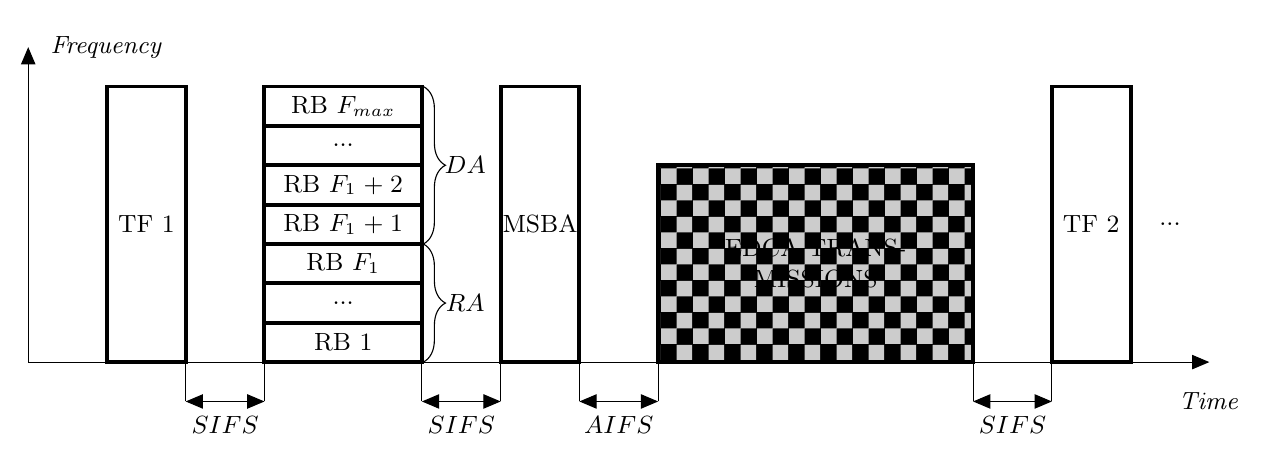
\begin{tikzpicture}
		\small
		
		\draw [arrows={-triangle 45}] (0,1) -- (15,1);
		\draw [arrows={-triangle 45}] (0,1) -- (0,5);
		\node at (15,  0.5) {\textit{Time}};
		\node at (1,  5) {\textit{Frequency}};
		
		\draw [line width=0.5mm] (1, 1) rectangle (2, 4.5);
		\node [text width=1.5cm, align=center] at (1.5,  2.75) {TF 1};
		
		\draw (2.0,  0.5) -- (2.0,  1.0);
		\draw (3.0,  0.5) -- (3.0,  1.0);
		\draw [arrows={triangle 45-triangle 45}] (2.0,0.5) -- (3.0,0.5);
		\node at (2.5, 0.2) {$SIFS$};
		
		\draw [line width=0.5mm] (3, 1.0) rectangle (5, 1.5);
		\draw [line width=0.5mm] (3, 1.5) rectangle (5, 2.0);
		\draw [line width=0.5mm] (3, 2.0) rectangle (5, 2.5);
		\draw [line width=0.5mm] (3, 2.5) rectangle (5, 3.0);
		\draw [line width=0.5mm] (3, 3.0) rectangle (5, 3.5);
		\draw [line width=0.5mm] (3, 3.5) rectangle (5, 4.0);
		\draw [line width=0.5mm] (3, 4) rectangle (5, 4.5);
		
		\node [text width=2cm, align=center] at (4, 1.25) {RB 1};
		\node [text width=2cm, align=center] at (4, 1.75) {...};
		\node [text width=2cm, align=center] at (4, 2.25) {RB $F_1$};
		\node [text width=2cm, align=center] at (4, 2.75) {RB $F_1+1$};
		\node [text width=2cm, align=center] at (4, 3.25) {RB $F_1+2$};
		\node [text width=2cm, align=center] at (4, 3.75) {...};
		\node [text width=2cm, align=center] at (4, 4.25) {RB $F_{max}$};
		
		\draw [decorate,decoration={brace,amplitude=8pt,mirror,raise=0.5pt},yshift=0pt]
		(5,1) -- (5,2.5) node [black,midway,xshift=0.55cm] {$RA$};
		\draw [decorate,decoration={brace,amplitude=8pt,mirror,raise=0.5pt},yshift=0pt]
		(5,2.5) -- (5,4.5) node [black,midway,xshift=0.55cm] {$DA$};
		
		\draw (5.0,  0.5) -- (5.0,  1.0);
		\draw (6.0,  0.5) -- (6.0,  1.0);
		\draw [arrows={triangle 45-triangle 45}] (5.0,0.5) -- (6.0,0.5);
		\node at (5.5, 0.2) {$SIFS$};
		
		\draw [line width=0.5mm] (6, 1) rectangle (7, 4.5);
		\node [text width=1.5cm, align=center] at (6.5,  2.75) {MSBA};
		
		\draw (7.0,  0.5) -- (7.0,  1.0);
		\draw (8.0,  0.5) -- (8.0,  1.0);
		\draw [arrows={triangle 45-triangle 45}] (7.0,0.5) -- (8.0,0.5);
		\node at (7.5, 0.2) {$AIFS$};
		
		\draw[draw = none,pattern=checkerboard light gray, pattern color=black] (8,1) rectangle (12,3.5);
		\draw [line width=0.5mm] (8, 1) rectangle (12, 3.5);
		\node [text width=3cm, align=center] at (10,  2.25) {EDCA TRANSMISSIONS};
		
		\draw (12.0,  0.5) -- (12.0,  1.0);
		\draw (13.0,  0.5) -- (13.0,  1.0);
		\draw [arrows={triangle 45-triangle 45}] (12.0,0.5) -- (13.0,0.5);
		\node at (12.5, 0.2) {$SIFS$};
		
		\draw [line width=0.5mm] (13, 1) rectangle (14, 4.5);
		\node [text width=3cm, align=center] at (13.5,  2.75) {TF 2};	
		\node [text width=1.5cm, align=center] at (14.5, 2.75) {...};
		
		\end{tikzpicture}}
	\caption{\label{fig:transmission} Frame handshake for UL OFDMA transmission (NEED TO CHECK).}
	\vspace{-0.5em}
\end{figure*}

UL OFDMA transmission is more challenging, since
OFDMA transmissions of each STAs shall start and end
simultaneously. That is why it starts with a trigger frame in
which the AP allocates RUs to each STA and informs the
STAs about the transmission parameters, e.g. MCS, transmission
duration. Being polled with the trigger frame, each
STA immediately replies with a data frame. The amendment
describes several ways how to meet the requirement on the
transmission duration. For example, advanced aggregation and
fragmentation methods, as well as padding, can be used. After
the UL transmission, the AP replies with a modified ACK
frame, in which the AP acknowledges successfully received
packets or fragments. To notify the AP that the STA has
some data for transmission, it can send a buffer status report
with the legacy channel access method, or as a part of the
described UL OFDMA transmission, or using ALOHA-like
Random OFDMA channel access, which is efficient only for
short transmissions and is not considered in the paper.

SIFS after TF reception, the STAs
transmit their parts of UL OFDMA frame. If needed, the
AP acknowledges reception of each part by sending a set of
ACKs inside an OFDMA frame or by sending Multi-STA
Block Acknowledgment (MSBA).
It is the AP which, for both DL and UL transmissions,
determines modulation and coding scheme (MCS), dura-
tion, RU assignment and other OFDMA parameters. Such
information can be transmitted in frame headers (for DL)
and in the Trigger frame (for UL). An example of UL
OFDMA transmission is shown in Fig. 2.
As mentioned above, 11ax moves decision making logic
from the STAs to the AP that determines which STA
transmits, when, in which RU, how much data it trans-
mits, etc. To make a correct decision, the AP needs to
be aware of STAs’ buffered traffic and channel conditions.
This information can be periodically requested by the
AP. Moreover, to notify the AP about arrived packets,
a STA can proactively send so-called Buffer Status Re-
port (BSR). For that, it can aggregate BSR with a data
frame sent in the dedicated RU. Another option is legacy
EDCA. Thanks to the recent change in the 11ax draft
standard, the AP can separately tune EDCA parameters
of scheduled STAs in such a way, that they do not contend
for the channel with unscheduled STAs. It means that
if a STA does not obtain UL RUs, it likely delivers a
BSR at the first transmission attempt because of the
extremely low contention. The third approach to send
a BSR is using OFDMA Random Access. For that, the
AP can allocate one or several RUs for random access
and the contending STAs will randomly choose one of
such RUs. Anyway, thanks to these methods, the AP can
quickly obtain information about new frames buffered at
the associated STAs and waiting for UL RUs.
OFDMA brings many benefits to 11ax networks. First
it makes transmission more reliable to frequency selec-
tive interference and fading. This is especially important
for wide 160 MHz channels introduced in 11ac. Second,
with OFDMA we can glue short packets destined for or
originated from various STAs, which significantly reduces
overhead caused by PHY headers and channel access time
and interframe spaces. Third, for UL transmissions by edge
STAs it makes sense to use narrow channels instead of wide
ones. Indeed, since the STAs are spatially separated they
can simultaneously transmit at the maximal allowed power
without breaking legal limitations on the emitted energy.
Thus, by reducing RU width, we increase power spectral
density received from the STAs and can use higher MCS.
In other words, by allowing numerous spatially separated
STAs to transmit in parallel, we increase the cumulative
received power in comparison to the case when only one
STA transmits. For edge STAs, increasing power spectral
density leads to a higher MCS, so the average amount
of data received from an OFDMA frame is higher than
that from a legacy. Thus in contrast to LTE, in 802.11ax
networks the rates in UL RUs are non-additive, i.e. if aSTA transmits in twice wider RU, it is not guaranteed that
it transmits twice more data. This effect will be carefully
investigated in the paper.

As it was described before STAs should pre-correct their transmission power in the following way. 
According to the 11ax standard, an AP indicates in the AP Tx Power  subfield in TF the combined transmit power $Tx^{AP}_{pwr}$ of all the transmit antennas used to transmit that TF normalized to 20 MHz bandwidth. 
Each STA that is allocated in the TF calculates UL transmit power $Tx_{pwr}^{STA}$ using:
\begin{equation}
Tx_{pwr}^{STA} = PL_{DL} + Target_{RSSI},
\end{equation}
where $Target_{RSSI}$ is taken from UI element and $PL_{DL}$ represents DL pathloss, which is computed by formula:
\begin{equation}
PL_{DL} = Tx^{AP}_{pwr} - DL_{RSSI},
\end{equation}
where $DL_{RSSI}$ represents measured received power from legacy preamble portion of TF. Both summands are normalized to 20MHz bandwidth. 

\section{Related Works}
\label{sec:related}
Despite the fact that 11ax is expected to be finished by 2019, it has been already studied a lot in the literature.

In \cite{lee-proportionalfair} authors try to adapt OFDMA schedulers in 3GPP LTE Uplink considering the contiguous allocation constraint appearing in those networks. They proved that scheduling problem with this condition is NP-Hard and offered some approximation algorithms to maximize proportional fair objective. However, when it comes to 11ax networks we should take into account additional condition that RU can consist only of specific number of tones so we cannot unite RUs in arbitrary way as it can be done in 3GPP LTE. 

It should be noted that 11ax has backward compatibility. 
However, when this standard will be released publicly and new generation of devices will come we could see legacy (pre 11ax) STAs suffering from this new amendment. 
In \cite{khorov2016several}, authors study the performance of the network consisting of the legacy and 11ax STAs. 
For this mixed network, authors offer a way to select optimal channel access parameter values, which guarantees fairness between legacy and 11ax STAs and significantly increases the number of the OFDMA transmissions for 11ax STAs.

\todo{rewrite}
Random access for UL OFDMA in 11ax has been studied in~\cite{lanante2017performance}. 
The authors consider STAs which have saturated data flows and use only random access mechanism for data transmission. 
For this scenario, they describe a mathematical model of transmission with OFDMA random access and use it for analysis and optimization of the 11ax network performance in terms of throughput and percentage of successful RUs. 
The methodology introduced in the paper might be used to tune the random access for OFDMA UL, however, usage of deterministic access is more feasible in terms of channel efficiency for the studied scenario.

Authors of \cite{sharon2017scheduling} explore multiple scheduling strategies by which a given number of stations can transmit over the UL in order to compare between the throughputs of 11ac and 11ax over the UL when considering UDP traffic and that several stations are transmitting in the system. However, the main goal of that paper is to show how much 11ax outperforms 11ac in terms of access delay and throughput with its novel mechanisms and ways to transmit. This paper does not offer any resource scheduler because authors assume that STAs are identical so it is pointless to distinguish them in resource priorities.  

\section{Network Scenario and Problem Statement}
\label{sec:scenario}

\begin{figure}[t]
	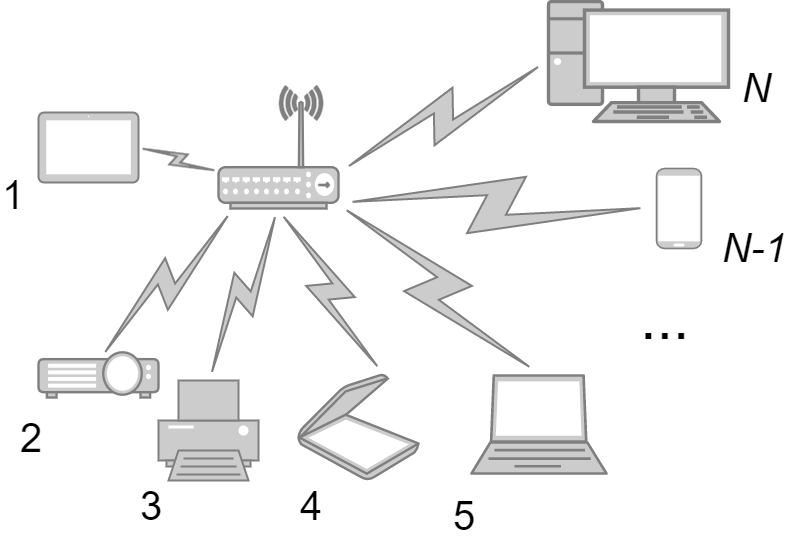
\includegraphics[width = 0.4\textwidth]{NetworkScenario}
	\caption{\label{fig:scenario} The network scenario}
\end{figure}

The considered Wi-Fi network scenario is shown in Fig~\ref{fig:scenario}. A group of $N$ STAs (STA) is associated to the Access point (AP). 
From time to time, STAs generate finite data flows to be delivered to the AP. Apart from that, we assume each STA to have only one flow.

We study UL scheduling problem in deterministic access, so let STAs transmit their BSR in EDCA transmissions period, so there is no need for AP to allocate resources for RA during trigger-interval.
Also we have several defined schedulers for deterministic access (which will be discussed later on). 
Let time unit be the period with which the AP broadcasts trigger-frames.
So each time unit scheduler allocates resources for associated users in a certain way.

Users' STAs are transmitting data in uplink using OFDMA. 
It means that STAs should transmit their data with synchronized MCS and that AP should choose this MCS and allocate RUs satisfying the OFMA features described above. 

The considered network operates in a \SI{40}{\MHz} channel at 5 GHz. Hence, we have RU location shown in Fig.~\ref{fig:resource_units}. 
Also correspondence of RUs and given rates is demonstrated at Table.~\ref{table:RUdatarate}.

Problem statement: \textit{to adapt known schedulers which work in traditional cellular networks to 11ax networks.}

\section{Scheduling in 11ax}
\label{sec:scheduling}

The problem of resource allocation is usually formulated as the following optimization task.
Consider a network described in section~\ref{sec:scenario}.
Each time unit, the AP runs defined scheduler which allocates $M$ RUs to some STAs in order to maximize some network-wide utility function~$U$, where $M$ is a total number of RUs in chosen set of RUs. 
For example, if scheduler chooses the following RU set: 242, 106, 26, 52, 26, 26-tones RUs to STAs then $M = 6$. 
Note that the utility function intuitively should be $U = U(RU set, allocation, mcs)$ here because as shown in section~\ref{sec:features} several performance indicators can vary greatly depending on allocation of RU set and chosen MCS.

As justified in \cite{andrews2010scheduling}, in multi resource unit systems like OFDMA, we can represent the utility function $U(t)$ in the following objective form
\begin{equation}
\label{eq:obj}
U(t) = \sum_{i = 1}^{N} \sum_{j = 1}^{M} x_i^j \lambda_i^j (t)
\end{equation}
where $x_i^j$ is an indicator which equals 1 if STA $i$ is assigned to RU $j$, and 0, otherwise, $\lambda_i^j$ is the scheduler metric value which client STA $i$ has in RU $j$ at time slot $t$. 

It is clear that if STA has no data to transmit right now then it is pointless for the AP to allocate RU for this station. Thus, for convenience we denote $n(t)$ as a number of STAs which have data to transmit at the moment $t$. Let us sort them in a specific way clarified by scheduler and let $i\in[1, n(t)]$ be the index of STA at the moment $t$. We can reduce the number of terms in the sum above by excluding STAs without data. Also for clearness we sort RUs in ascending order.

For shortness, $X$ is the two-dimensional matrix of $\left\{x_i^j\right\}$ representing RU assignment to the STAs and $C = \{1\dots12\}$ be the set of all MCSs (according to the table~\ref{table:RUdatarate}). Let $R$ be the set of all RU configurations. With all aforementioned instructions we can rewrite common optimization problem for fixed RU set $r \in R$ and fixed MCS $c \in C$ for all possible scheduler metrics:
\begin{align} \label{eq:usl311}
\max U_{c, r}(t,X) = \max \sum^{n(t)}_{i = 1} \sum_{j = 1}^{M} x_i^j \lambda_i^j(t); \\ \label{eq:usl312}
\text{subject to} \sum_{i=1}^{n(t)} x_i^j \leq 1,\ \  \forall j \in [1,M]; \\ \label{eq:usl313}
\sum_{j = 1}^{M} x_i^j \leq 1, \ \ \forall i \in [1, n(t)]; \\ \label{eq:usl314}
\sum_{i = 1}^{n(t)} \sum_{j = 1}^{M} x_i^j \leq M,
\end{align}
where conditions~\eqref{eq:usl312}--\eqref{eq:usl314} are related to the OFDMA  constraints described before. 
Namely, \eqref{eq:usl312} represents the fact that one STA cannot be assigned to more than one RU. Condition \eqref{eq:usl313} works in opposite way: one RU cannot be assigned for more than one station. The last condition \eqref{eq:usl314} comes with a total number $M$ of RUs in this fixed RU set.

This problem is known as the assignment problem, which can be resolved in polynomial time using dynamic programming algorithm named as the Hungarian algorithm,~\cite{bourgeois1971extension}.
It is also known as the Kuhn-Munkers algorithm. 
Its solution is the assignment $\hat X$, which gives maximum value of $U_{c, r}(t,X)$  for any possible allocation matrix $X$ with fixed RU set and MCS. 
Briefly, the algorithm makes up the matrix $\Lambda = \{\lambda_i^j\}$ and chooses the best $\lambda_i^j$ in each line in order to maximize objective function \ref{eq:usl311}. Example is given in Fig.~\ref{fig:matrixexm} where grey cells of this matrix describe solution $\hat X$. 

With this algorithm the AP can allocate a fixed RU set with a fixed MCS, but it needs to determine them as well. The best RU set and the best MCS can be chosen among all possible variants by considering them one by one. This is final decision made by the AP. 
\textcolor{prpl}{It should be noted that there is not so many possible RU sets that its examination is quite feasible.}
The examination of RU set can be hastened by excluding configurations that are obviously worse than the known alternatives, and the examination of MCS should consider only supported MCSs and can be hastened by excluding MCSs lower than the highest MCS supported by all stations. It means that we have borders for MCS: $mcs^{*}_{min}$ and $mcs^{*}_{max}$. Let us introduce pseudo-coded Algorithm~\ref{alg:11ax} for 11ax resource scheduler 

\begin{algorithm}
	\caption{General 11ax scheduler algorithm}\label{alg:11ax}
	\begin{algorithmic}[1]
		\Procedure{Scheduler}{}
		\For{$r$ in $\{R\}$}
		\For{$c$ in $[mcs^{*}_{min};mcs^{*}_{max}]$}
		\State $\hat X = HungarianAlg(\Lambda(r, c))$
		\If {$U_{best} < U(\hat X)$}
		\State $U_{best} = U(\hat X)$,
		\State $X_{best} = \hat X$,
		\State $c_{best} = c$,
		\State $r_{best} = r$.
		\EndIf
		\EndFor
		\EndFor
		\State \Return $r_{best}$, $c_{best}$, $X_{best}$
		\EndProcedure
	\end{algorithmic}
\end{algorithm}

\begin{figure}[t]
\centering
\caption{\label{fig:matrixexm} Example on Hungarian algorithm}
\resizebox{0.8\columnwidth}{!}{
\setlength\tabcolsep{4pt} % default value: 6pt
\begin{tabular}{|c|c|c|c|c|c|c|c|c|c|c|c|}
\hline
$x_i^j$& \multicolumn{10}{|c|}{Client Stations, $i$}  \\\hline
\parbox[t]{2mm}{\multirow{7}{*}{\rotatebox[origin=c]{90}{Resource Units, $j$}}} & 2 & 2 & 3 & 6 & 7 & 1 & 3 & \cellcolor{gray!100}6 & 2 & 6 \\\cline{2-11}
& 1 & 4 & 5 & 8 & \cellcolor{gray!100}9 & 5 & 3 & 8 & 5 & 1 \\\cline{2-11} 
& \cellcolor{gray!100}9 & 4 & 7 & 5 & 3 & 2 & 6 & 1 & 3 & 1 \\\cline{2-11}
& 2 & 3 & 8 & 4 & 5 & 6 & 1 & 2 & \cellcolor{gray!100}7 & 4 \\\cline{2-11} 
& 7 & 4 & \cellcolor{gray!100}9 & 3 & 7 & 1 & 2 & 8 & 5 & 8 \\\cline{2-11}
& 9 & 7 & 4 & \cellcolor{gray!100}7 & 8 & 2 & 2 & 4 & 3 & 6 \\\cline{2-11}
& 9 & \cellcolor{gray!100}8 & 5 & 6 & 1 & 2 & 4 & 5 & 6 & 7 \\\hline
\end{tabular}
}
\end{figure}

\section{Ax-adaptations of Known Schedulers}
\label{sec:adaptations}

The most widely used utility functions and corresponding schedulers are listed below. For shortness, let us write $n$ instead of $n(t)$.

\subsection{Max Rate}

The AP in legacy Wi-Fi and Base Station (BS) in cellular networks use the Max Rate (MR) scheduler in order to maximize  throughput $S(t)$ at current moment $t$. This scheduler considers all client stations and assigns the whole frequency band to a station with the highest nominal data rate $r_i$ of station $i$ in channel.

Scheduler in classic Wi-Fi сan distribute only a time resource.
However, with appearance of 11ax standard the AP can consider channel frequency division too and maximize cumulative throughput $S(t) = \sum S_i(t)$, where $S_i(t)$ is throughput of station $i$ at time instant $t$. We should simply make   
\begin{equation}
\label{eq:lambdamr}
\lambda_i^j (c) = r_i^j (c),\ i \in [1,N],\ j \in [1, M].
\end{equation}
With this equation we get objective function~\eqref{eq:usl311} in a form:
\begin{equation}
\label{eq:11axmrutility}
U^{MR}_{c,r}(t,X) = \sum_{i = 1}^{n} \sum_{j = 1}^{M} r_i^j (c)
\end{equation}
maximization of which obviously gives us allocation with the biggest rate for fixed RU set. Thus, 11ax-MR scheduler should solve \eqref{eq:usl311}--\eqref{eq:usl314} with parameter \eqref{eq:lambdamr}.

\subsection{Proportional Fair}

The Proportional Fair (PF) scheduler allocates RUs to the STAs in a way which maximizes 
\begin{equation}
\label{eq:11axpfutility}
U_{c,r}^{PF} = \sum_{i=1}^{n}\sum_{j=1}^{M} x_i^j \frac{r_i^j}{Q_i}
\end{equation}
in a time domain, where $Q_i$ is the average service rate, e.g. amount of data transmitted by the STA $i$ divided by its total time in system. This utility function is fully analogous to the objective function \eqref{eq:obj} with
\begin{equation}
\label{eq:pflambda}
\lambda_i^j (c) = \begin{cases}
\frac{r_i^j(c)}{Q_i},\ if\ Q_i \ne 0,\\
0,\ otherwise;
\end{cases}
\end{equation}

In cellular networks PF algorithms usually consider each RU one-by-one, i.e. for RU $j$ it allocates user who maximizes $r_i^j / Q_i$ at time slot $t$. But in a classic Wi-Fi there is only one RU --- the whole channel itself. So we assume that PF in legacy Wi-Fi works only with this RU.

In cellular networks this exhaustive search over each RU can be feasible due to fact that all RUs are equal to each other. This assumption is not met in 11ax networks, so the 11ax-PF AP should solve optimization task~\eqref{eq:usl311}--\eqref{eq:usl314} with parameter~\eqref{eq:pflambda}.


\subsection{Shortest Remaining Time First}

If the channel properties do not change with time and the rate in different RUs is the same and additive, the Shortest Remaining Time First (SRTF) scheduler is proven to provide minimal average upload time. 
The second assumption made to derive such a scheduler is completely incorrect for UL OFDMA transmission in 11ax networks.

But still, simplistically, in classic Wi-Fi and in cellular networks SRTF allocates the whole channel to a user for which $\theta_i=\frac{D_i(t)}{r_i}$ is the minimal one, where $D_i(t)$ is the remaining amount of data of user $i$ and as before $r_i$ is its rate in the whole channel. 
In other words this scheduler sorts STAs by parameter $\theta_i$ and gives all resources to the first one in this sorted list. 

In this case, the first STA finishes delivering its flow by time $\theta_1$ except for waiting.
The second STA starts right after the first one and delivers its flow by time $\theta_2 + \theta_1$, etc. and as a result total upload time would be
\begin{multline}
\label{eq:srtfuploadtime}
T_{SRTF} = n\cdot\theta_1 + (n-1)\cdot\theta_2 + (n-2)\cdot\theta_3 + \dots \\ \dots + \theta_n = \sum_{i = 1}^n (n - i + 1) \theta_i.
\end{multline}

So, it is obvious this time would be minimal when we sort the STAs in the ascending order by $\theta_i$ when conditions are met.

Actually, 11ax adaptation of this scheduler is not a trivial task. So in this subsection we design a novel family of 11ax schedulers called 11ax-SRTF or MUTAX, Minimizing Upload Time in 11ax networks based on classic SRTF. Transmission process with SRTF scheduler is shown in Fig.~\ref{fig:SRTF}.
While deriving formula we neglect the effects related to packetization (including aggregation and fragmentation) overhead. 

Let slot be a time interval between two consequent TFs.
It should be noted that slots may have different duration. The maximal one is related to the standard limit of \SI{5484}{\us} for the physical protocol data unit (PPDU) duration. A slot can be shorter, if at least one STA which transmits in this slot has no more data.

The MUTAX algorithm has two steps. At the first step, we calculate the sum upload time of the flows, as if we used legacy SRTF scheduler, given by formula~\eqref{eq:srtfuploadtime}.

At the second stage, we try to improve results from assumption that we are using only the whole channel by serving some flows in parallel for the nearest slot. So, we divide the channel into several RUs according to some RU~set. For the clearness, see Fig.~\ref{fig:mutex}.

With defined notations in previous section, the total upload time $T_{MUTAX}\left(X\right)$ of existing flows differs from $T_{SRTF}$ in the following way. First, the upload time of each of $n$ flows increases by the current slot duration $\tau$. Second, if $x_i^j=1$, the remaining amount of data of flow $i$ decreases by the amount of data the STA~$i$ transmits in RU~$j$ of the current slot: $\Delta D_i^j = \min\left\{D_i, \tau \times r_{i}^{j}\right\}$. Thus,  
\begin{equation}
T_{MUTAX}\left(X\right) = n \tau + \sum_{i = 1}^{n} \left(n - i\right) \frac{D_i -  \sum_{k = 1}^{M} x_i^j \Delta D_i^j}{r_{i}}
\end{equation}

Since both $\tau$ and  $\Delta D_i^j$ depend on the resource allocation $X$, minimization of $T_{MUTAX}(X)$ requires exhaustive search by possible ways to allocate the RUs to the STAs like we have offered in previous section, and to simplify the task we propose an heuristic approach based on two assumptions.
Firstly, we neglect the change of $n \tau_t$ for different allocations, as a slot cannot be too long due to standard limitations.
Secondly, we sort the STAs in the ascending order by $t_n$ only once, before considering different ways to assign RUs to the STAs.
Under these assumptions, to minimize  $T(X)$, we have to maximize the following expression 
\begin{equation}
\label{eq:11axsrtfutility}
U_{c,r}^{MUTAX} = 
\sum_{i = 1}^{n} \sum_{j = 1}^{M } \left(n - i\right) \frac{x_i^j \Delta D_i^j}{r_{i}}.
\end{equation}
which gives us utility function of this scheduler. Finally, let us denote 
\begin{equation}
\label{eq:lambdasrtf}
\lambda_i^j = \left(n - i\right) \frac{\Delta D_i^j}{r_{i}}
\end{equation}
using which we can define the following optimization problem \eqref{eq:usl311}--\eqref{eq:usl314} with parameter~\eqref{eq:lambdasrtf}.

We can improve this approach to schedule current slot in assumption that afterwards it will work under legacy scheduler which allocates the whole channel. Note that the AP has no need to reschedule resources with new TF unless new STA comes with new data to transmit or a STA ends its transmission during the last TF slot. This idea is illustrated in Fig.~\ref{fig:mutexso}. Thus, The AP can leave the allocation of resources the same until the above conditions are met. 

\begin{figure}[tb]
	\centering
	\footnotesize
	\begin{scaletikzpicturetowidth}{\columnwidth}
		\begin{tikzpicture}[scale = \tikzscale]
		\draw[draw = none, pattern= north east lines, pattern color=black, ] (1.4,1) rectangle (3,3);
		
		\draw[draw = none, pattern=checkerboard light gray, pattern color=black, ] (3,1) rectangle (5,3);
		
		\draw[draw = none, pattern=dots, pattern color=black, ] (5,1) rectangle (8.5,3);
		
		\draw (1.4,3) -- (1.4,1);
		\draw (3,3) -- (3,0.75);
		\draw (5,3) -- (5,0.75);
		\draw (8.5,3) -- (8.5,0.75);
		
		\draw [arrows={-triangle 45}] (-0.5,1) -- (12,1);
		
		\draw [arrows={-triangle 45}] (0.2,1) -- (0.2,3.7);
		
		\node at (12,  1.3) {\textit{Time}};
		\node at (1.3,  3.5) {\textit{Frequency}};
		
		\node at (2.2,2) {\textbf{STA 1}};
		\node at (4,2) {\textbf{STA 2}};
		\node at (6.7,2) {\textbf{STA 3}};
		
		\scriptsize
		\node at (3,  0.55) {$t_1$};
		\node at (5,  0.55) {$t_1+t_2$};
		\node at (8.5,  0.55) {$t_1+t_2 + t_3$};
		
		\end{tikzpicture}
	\end{scaletikzpicturetowidth}
	\caption{\label{fig:SRTF} Workflow of SRTF scheduler}
	
	\vspace{0.5cm}
	
	\begin{scaletikzpicturetowidth}{\columnwidth}
		\begin{tikzpicture}[scale = \tikzscale]
		\draw[draw = none, pattern=north east lines, pattern color=black, ] (1.4,2) rectangle (2.6,3);
		\draw[draw = none, pattern=checkerboard light gray, pattern color=black, ] (1.4,1.56666) rectangle (2.6,2);
		\draw[draw = none, pattern=dots, pattern color=black, ] (1.4,1.12222) rectangle (2.6,1.56666);
		
		\node at (2,2.5) {\textbf{1}};
		\node at (2,1.8) {\textbf{2}};
		\node at (2,1.3) {\textbf{3}};
		
		\draw[draw = none, pattern=north east lines, pattern color=black, ] (2.6,1) rectangle (3.4,3);
		\node at (3,2) {\textbf{1}};
		\draw[draw = none, pattern=checkerboard light gray, pattern color=black, ] (3.4,1) rectangle (5.2,3);
		\node at (4.25,2) {\textbf{STA 2}};
		\draw[draw = none, pattern=dots, pattern color=black, ] (5.2,1) rectangle (8,3);
		
		\draw [arrows={-triangle 45}] (-0.5,1) -- (12,1);
		
		\draw [arrows={-triangle 45}] (0.2,1) -- (0.2,3.7);
		
		\draw (2.6,3) -- (2.6,0.75);
		\draw (3.4,3) -- (3.4,0.75);
		\draw (5.2,3) -- (5.2,0.75);
		\draw (8,3) -- (8,0.75);
		
		\node at (12,  1.3) {\textit{Time}};
		\node at (1.3,  3.5) {\textit{Frequency}};
		
		\node at (6.5,2) {\textbf{STA 3}};
		
		\scriptsize
		\node at (2.42,0.5) {\vphantom{$\tilde t_1$} $\tau$};
		\node at (3.4,0.5) {$\tau+\tilde t_1$};
		\node at (5.2,0.5) {$\tau+\tilde t_1 + \tilde t_2$};
		\node at (8,0.5) {$\tau+ \tilde t_1 + \tilde t_2+ \tilde t_3$};
		\end{tikzpicture}
	\end{scaletikzpicturetowidth}
	\caption{\label{fig:mutex} Workflow of MUTAX scheduler}
	
	\vspace{0.5cm}
	
	\begin{scaletikzpicturetowidth}{\columnwidth}
		\begin{tikzpicture}[scale = \tikzscale]
		\draw[draw = none, pattern=north east lines, pattern color=black, ] (1.4,2) rectangle (3.1,3);
		\draw[draw = none, pattern=checkerboard light gray, pattern color=black, ] (1.4,1.56666) rectangle (3.1,2);
		\draw[draw = none, pattern=dots, pattern color=black, ] (1.4,1.12222) rectangle (3.1,1.56666);
		
		\draw[draw = none, pattern=checkerboard light gray, pattern color=black, ] (3.1,1) rectangle (4.9,3);
		\node at (4,2) {\textbf{STA 2}};
		\draw[draw = none, pattern=dots, pattern color=black, ] (4.9,1) rectangle (7.8,3);
		
		\node at (2.2,2.5) {\textbf{1}};
		\node at (2.2,1.8) {\textbf{2}};
		\node at (2.2,1.3) {\textbf{3}};
						
		\draw [arrows={-triangle 45}] (-0.5,1) -- (12,1);
		
		\draw [arrows={-triangle 45}] (0.2,1) -- (0.2,3.7);
		
		\draw (3.1,3) -- (3.1,0.75);
		\draw (4.9,3) -- (4.9,0.75);
		\draw (7.8,3) -- (7.8,0.75);
		
		\node at (12,  1.3) {\textit{Time}};
		\node at (1.3,  3.5) {\textit{Frequency}};
		
		\node at (6.35,2) {\textbf{STA 3}};
		
		\scriptsize
		\node at (3.1,0.5) {\vphantom{$\tilde t_1$} $\tau^*$};
		\node at (4.9,0.5) {$\tau+\tilde t_2$};
		\node at (7.8,0.5) {$\tau+ \tilde t_2 + \tilde t_3$};
		\end{tikzpicture}
	\end{scaletikzpicturetowidth}
	\caption{\label{fig:mutexso} Workflow of MUTAX-SO scheduler}		
\end{figure}

But in this case we should change a bit the previous optimization task. Now we have the recent $n^* = n\tau\cdot\lceil\frac{\tau^*}{\tau}\rceil$, where $\tau^*$ is time until which a STA ends its transmission. In other words, it is minimal transmission length among all. We should divide it by $\tau$ and ceil up, so we get quantity of slots which are wasted by all associated STAs. We cannot obtain that parameter directly since it depends on the final RU set choice and its allocation, but we can make 1 step ahead and try to compute the smallest transmission time among all the STAs in the smallest RU. We also need to change the subtracted part in numerator to satisfy changes in. So it should be multiplied by $\lceil\frac{\tau^*}{\tau}\rceil$ for because STAs is planned to transmit this data for increased amount of slots. Finally, we get $D_i^{j*} = \min\left\{D_i, \tau\cdot\lceil\frac{\tau^*}{\tau}\rceil \times r_{i}^{j}\right\}$. Thus,  
\begin{equation}
\label{eq:timesrtfso}
T\left(X\right) = n^* \tau + \sum_{i = 1}^{n} \left(n - i\right) \frac{D_i -  \sum_{k = 1}^{M} x_i^j \Delta D_i^{j*}}{r_{i}}
\end{equation}

So analogically we get the same metric for the \eqref{eq:usl311}--\eqref{eq:usl314} task.
\begin{equation}
\label{eq:lambdasrtfso}
\lambda_i^j = \left(n - i\right) \frac{\Delta D_i^{j*}}{r_{i}}
\end{equation}

Additionally, we can try to calculate the desired time given by formula $\eqref{eq:timesrtfso}$ and search minimum among all RU sets. Thus, here we can define utility function:
\begin{multline}
\label{eq:ulilitysrtfso}
U_{c,r}^{MUTAX\text{-}SO} = -\Biggl[ n^* \tau +\\
+ \sum_{i = 1}^{n} \left(n - i\right) \frac{D_i -  \sum_{k = 1}^{M} x_i^j \Delta D_i^{j*}}{r_{i}}\Biggr]
\end{multline}
instead of $\sum \lambda x$. So here the AP solves \eqref{eq:usl311}-\eqref{eq:usl314} task with \eqref{eq:lambdasrtfso} and after it in that pseudo code it uses \eqref{eq:ulilitysrtfso} in the last condition part.
\section{Numerical Results}
\label{sec:numerical}

\begin{figure*}[tb]
	\centering
	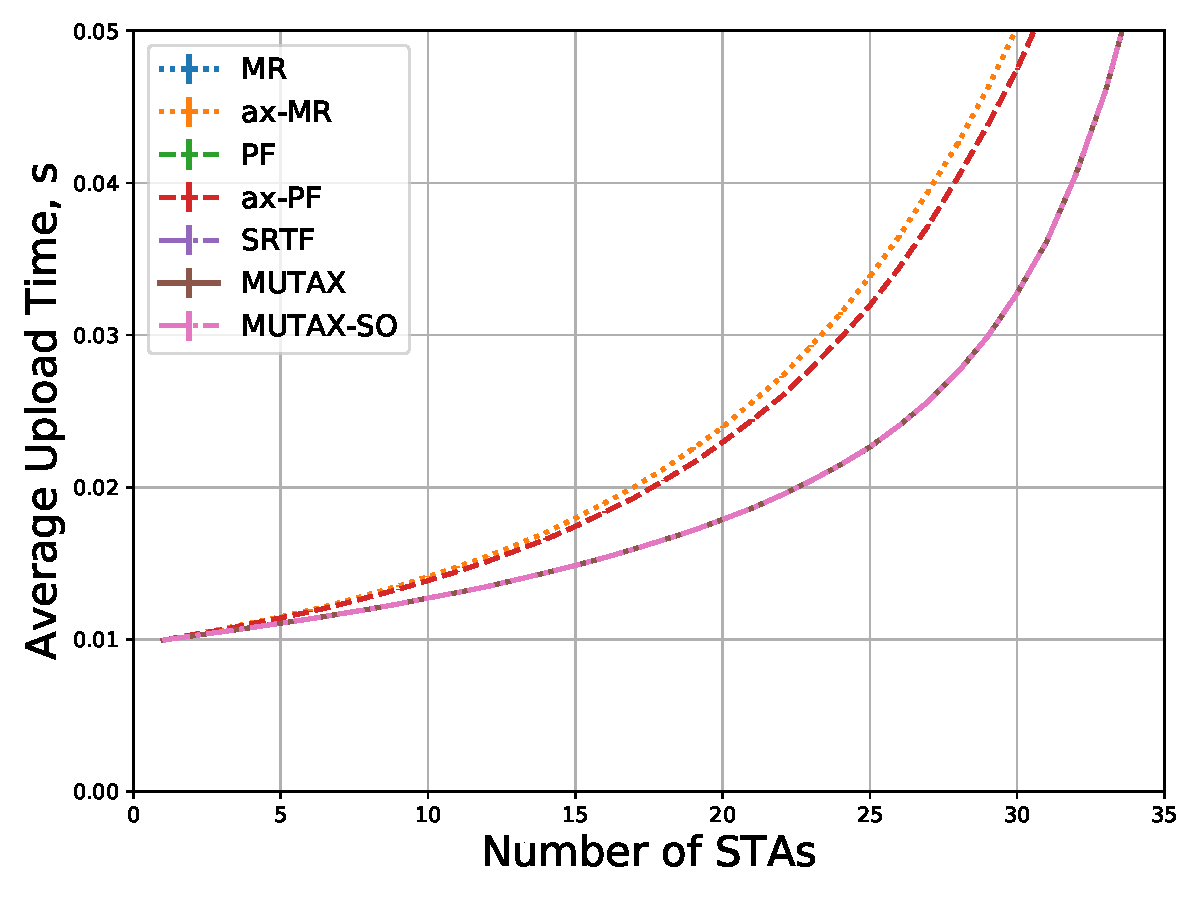
\includegraphics[width = 0.329\textwidth]{5-d.pdf}
	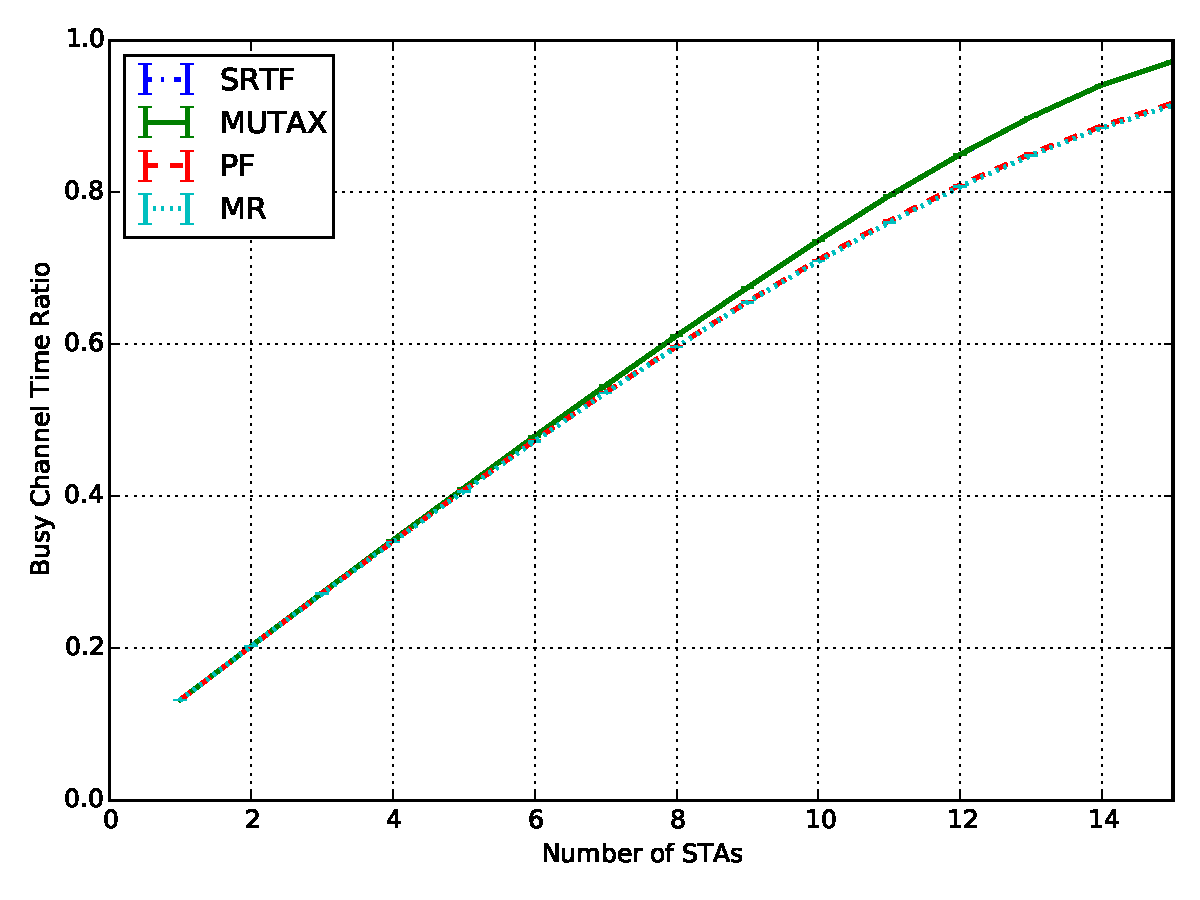
\includegraphics[width = 0.329\textwidth]{5-e.pdf}
	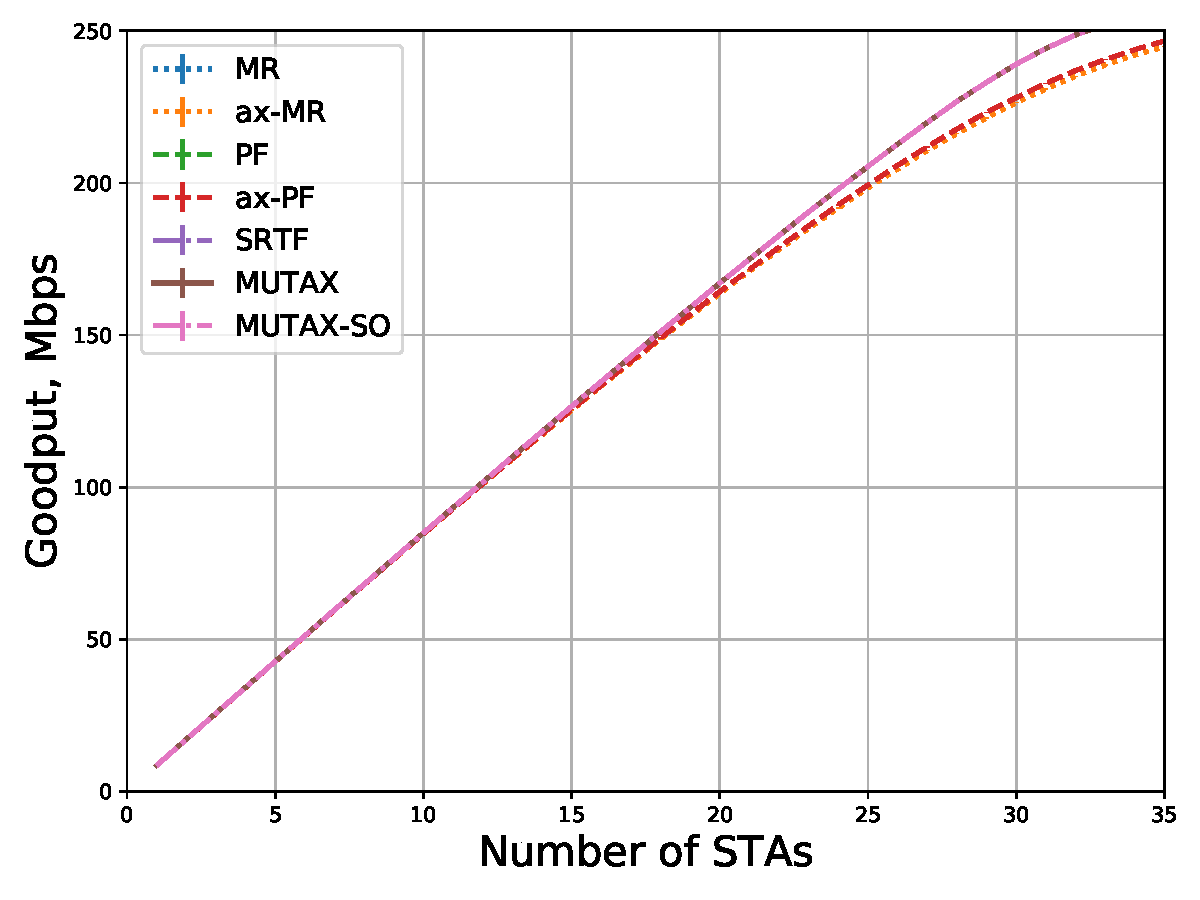
\includegraphics[width = 0.329\textwidth]{5-t.pdf}
	\caption{\label{fig:10metres}  Upload time, busy channel time ratio and goodput vs the number of STAs in the small circle.}
\end{figure*}

\begin{figure*}[bt]
	\centering
	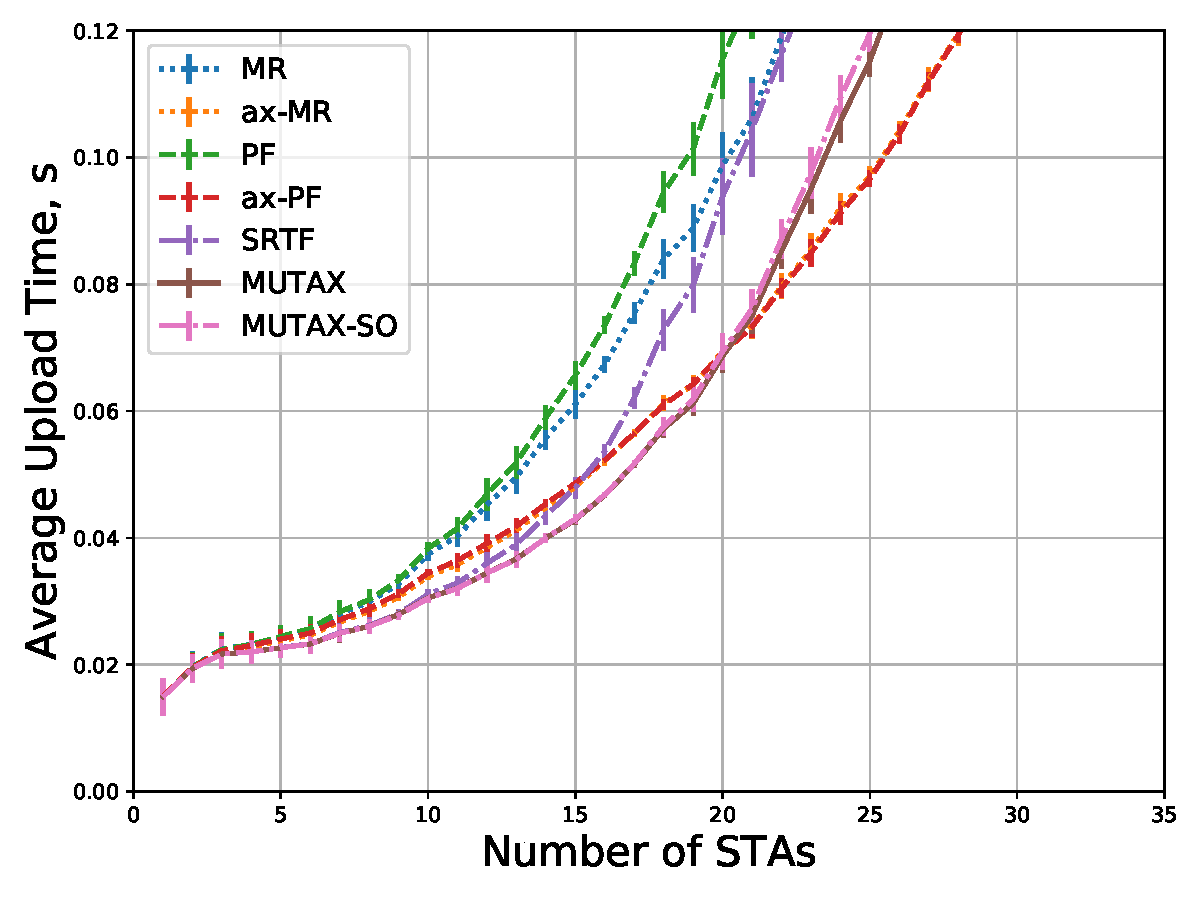
\includegraphics[width = 0.329\textwidth]{20-d.pdf}
	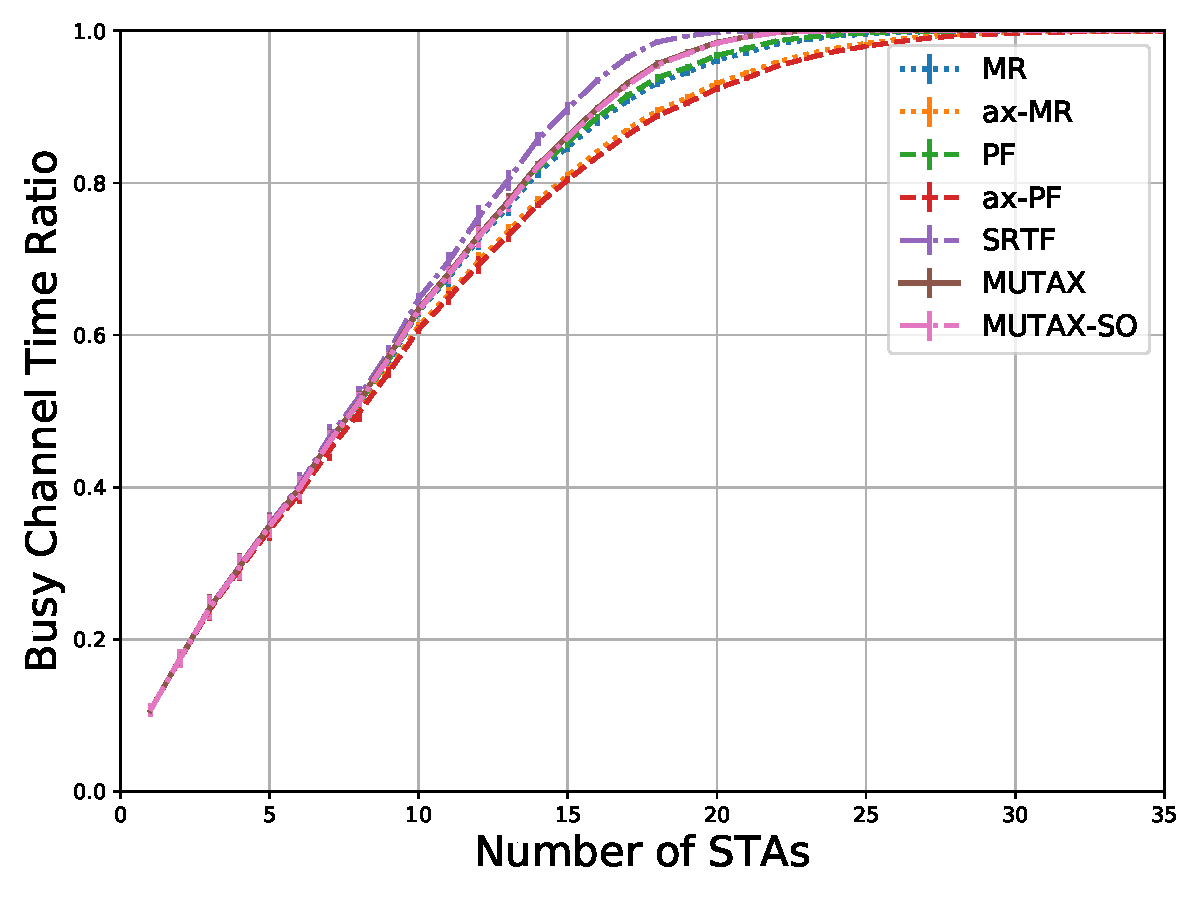
\includegraphics[width = 0.329\textwidth]{20-e.pdf}
	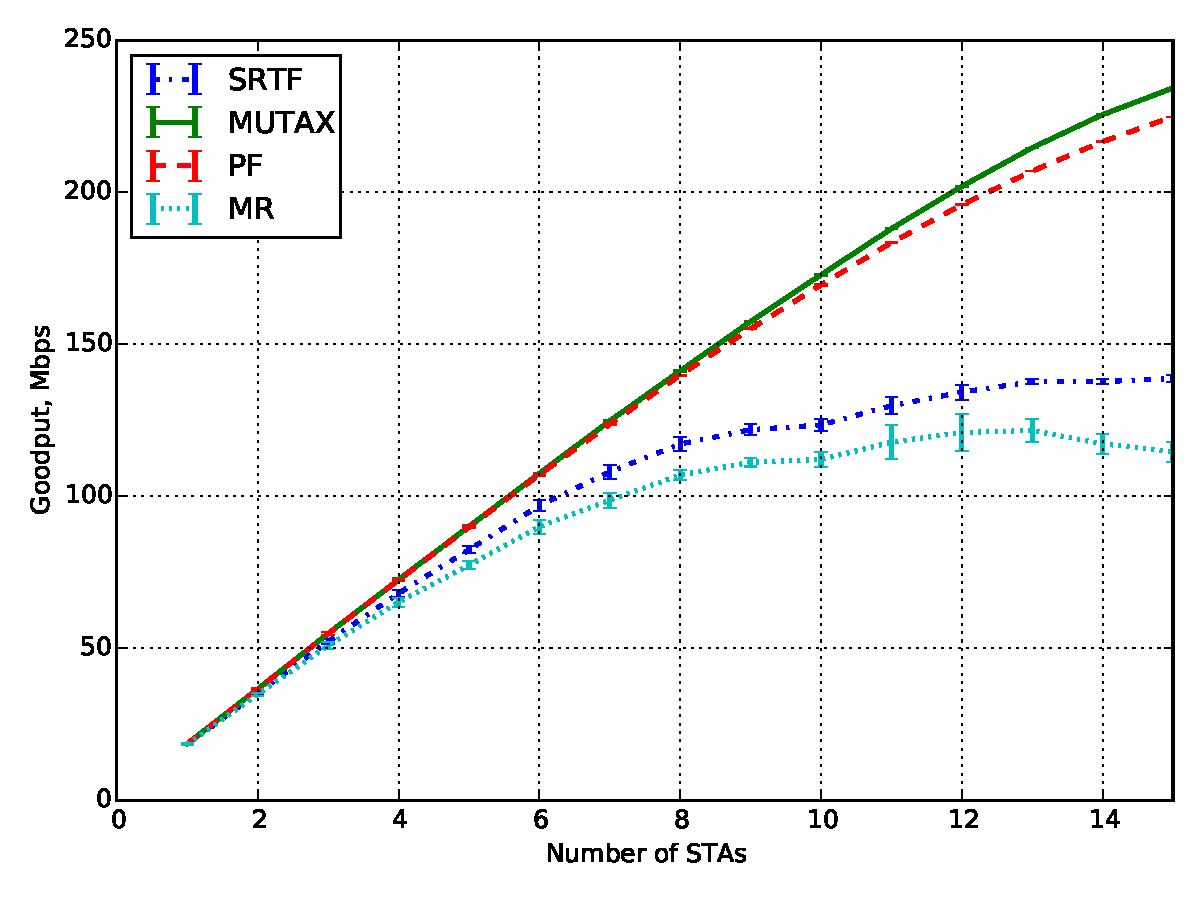
\includegraphics[width = 0.329\textwidth]{20-t.pdf}
	\caption{\label{fig:20metres} Upload time, busy channel time ratio and goodput vs the number of STAs in the large circle.}
\end{figure*}

We have implemented SRTF, MR and PF schedulers as well as 11ax analogs described in the previous section.

We run simulation in a scenario described in Section \ref{sec:scenario}.

The flow sizes are drawn from truncated lognormal distribution with minimal, average and maximal values of 1 KB, 200 KB, 3 MB respectively. 
When a flow is delivered, the next flow is generated after a random delay drawn from truncated exponential distribution with minimal, average and maximal values of \SI{0.1}{\s}, \SI{0.3}{\s} and \SI{0.6}{\s} respectively.
Also we used the following 802.11ax path-loss model for the residential scenario \cite{presentation_scenarios}:
\begin{multline*}
PL(d) = 40.05 + 20 \lg\left(\frac{f_c}{2.4}\right) + 20 \lg(\min(d, 5)) + \\
+ \mathbb{I}(d > 5) \cdot 35 \lg\left(\frac{d}{5}\right),
\end{multline*}
where $PL$ is the path-loss in dB, $f_c$ is the central frequency in GHz, $d$ is the distance between the devices and $\mathbb{I}{(x) }$ equals $1$ if $x$ is true and $0$ otherwise.
The AP receives the signal from the STAs with power $P(d)$ calculated as
$$
P(d) = P_0 + 10 \lg\left(\frac{F}{F_{max}}\right) - PL(d),
$$
where $P_0$ is the STA's transmission power, possibly corrected as mentioned in Section~\ref{sec:features}, $d$ is the distance between the STA and the AP, $F$ is the number of tones in the RU, and $F_{max}$ is the maximal number of tones in a RU in the considered channel.

In the first set of experiments, the STAs are located uniformly within a small circle of radius $\rho = \SI{5}{\m}$ around the AP.
In such a case, the channel quality is so high that the all STAs use the maximal MCS to transmit in given RU of any width.
Obviously, in this case OFDMA cannot bring any profit against legacy Wi-Fi which uses the whole channel for transmissions, as its division without changing the MCS cannot increase the data rate according to the Table~\ref{table:RUdatarate} unless MCS  can cope with the noise. The only possible exception here is ax-PF scheduler which tries to serve STAs with fairness, but actually multiplier $r^j_i (c)$ is a lot larger for $c=12$ in 484-tone~RU, compared to other RUs, so even 11ax-PF scheduler decides to allocate the whole channel to one user (need to check).

This result is supported by simulation, see Fig~\ref{fig:10metres}, which shows that if the channel for all STAs is good enough, schedulers which consider channel division yield the same upload time as others (curves coincide for them in this Fig.). Also this result illustrates that schedulers belonging to SRTF-family outperform the PF and MR-families by up to 30\%. 

As we consider traffic model of a closed loop system, along with the reduction of upload time SRTF-based schedulers provide the increase of goodput compared to the other schedulers.

The second set of experiments corresponds to the case when STAs are located in a larger circle of radius $\rho = \SI{20}{\m}$.
Such conditions provide a variety in MCS choice among STAs and RU widths, so it becomes possible to get gain from division the channel between different users.

If in previous set of experiments we could divide schedulers by their family belonging, here OFDMA usage is the main factor of success.
According to simulation results, see Fig.~\ref{fig:20metres}, in this case non-OFDMA schedulers are  much less efficient than channel-splitting schedulers. 
The gap between these two groups increases with the number of client STAs. 
Thus, usage of OFDMA gives advantage compared to non-OFDMA schedulers. 
\textcolor{prpl}{For example, designed to minimize upload time the classic SRTF does its job worse than 11ax adaptation of PF which was not developed for this purpose.}
At the same time, MUTAX and its SO version shows approximately the same upload time as ax-PF and ax-MR, they keep leading position unless number of STAs is less than 20.  

\section{Conclusion}
\label{sec:conclusion}

In the paper, we have studied scheduling problem in 11ax networks, the standard of which is currently under development. We have shown the constraints connected to a OFDMA usage and common approach to all possible schedulers for 11ax network.
Also we have demonstrated how classic schedulers can be adapted to 11ax networks and numerical results about their performance. 
Meanwhile, a new family of schedulers based on traditional SRTF scheduler was introduced. 
We can admit that MUTAX and MUTAX-SO make some brutal force optimization, they even start to lose to 11ax adaptations of PF and MR with increase in number of associated STAs. 
Thus, this problem should be investigated more deeply, but the main point of this paper stands that the AP can get gain in performance indicators due to division of channel.

\bibliographystyle{IEEEtran}
\bibliography{biblio} 
\end{document}
